\section{Problem Set 5}
\subsection{Control Objectives} \label{sec:control_objectives}
\subsubsection{Operational Modes}
The ultimate goal of our formation is to demonstrate on-orbit servicing of an uncontrollable target spacecraft with a swarm of one docking satellite and one observing satellite. Specifically, the Target spacecraft (SV1) has no maneuvering capabilities as it has run out of propellant, and our formation is aiming to refuel it. As such, SV1 will act as the origin of the RTN frame and remain there throughout all of our operational modes. The Watcher spacecraft (SV2) has sensing capabilities, including optical cameras such as those in the NASA Starling mission, which will be used to inspect the Target and estimate its pose for servicing purposes. The Docker spacecraft (SV3) also has optical sensors that will aid in this inspection, but also play a crucial role in proximity and docking operations. Our formation aims to demonstrate a significant advance in on-orbit pose estimation and characterization of objects, along with improved docking operations through the use of multiple spacecraft with a variety of sensor modalities. 

In order to achieve this, the significant operational modes of our formation are as follows: 

\begin{enumerate}
\item \textbf{Initial Checkout Mode} - Initial checkout of Target spacecraft with both Watcher and Docker less than a kilometer and more than 200 meters away at closest approach to allow for vision-based sensing
\item \textbf{Approach Mode} - Docker approaches the Target while Watcher watches from the same distance. This mode runs until the Docker is approximately 10 meters away from the Target
\item \textbf{Proximity Operations Mode} - Docker completes final approach Target while Watcher watches
\item \textbf{Docked Mode} - Docker docks and services Target while Watcher watches
\item \textbf{Station Keeping Mode} - Watcher and Target stay within prescribed limits of relative eccentricity and relative inclination to remain passively safe. This mode will be applied whenever the formation is not reconfiguring. 
\end{enumerate}

\subsubsection{Operational Mode ROEs}
The absolute motion of our spacecraft is not the focus, as our formation is purely concerned with servicing a satellite. As such, all of the operational modes are defined as deputy ROEs as follows. Note that the Approach mode was split into two separate waypoints (Mode 2 and Mode 3) to better illustrate the reconfiguration. 

\begin{table}[h!]
\centering
\begin{tabular}{|c|rrrrrr|rrrrrr|}
\hline
\textbf{Mode} & \multicolumn{6}{c|}{\textbf{SV2 (m)}} & \multicolumn{6}{c|}{\textbf{SV3 (m)}} \\
\cline{2-13}
 & $d_a$ & $d_\lambda$ & $d_{e_x}$ & $d_{e_y}$ & $d_{i_x}$ & $d_{i_y}$ 
 & $d_a$ & $d_\lambda$ & $d_{e_x}$ & $d_{e_y}$ & $d_{i_x}$ & $d_{i_y}$ \\
\hline
1 & 0 & 0 & 0 & 300 & 0 & 300 & 0 & 0 & 0 & 250 & 0 & -250 \\
2 & 0 & 0 & 0 & 300 & 0 & 300 & 0 & 0 & 0 & 100 & 0 & -100 \\
3 & 0 & 0 & 0 & 300 & 0 & 300 & 0 & 0 & 0 & 10  & 0 & -10 \\
4 & 0 & 0 & 0 & 300 & 0 & 300 & 0 & 0 & 0 & 1   & 0 & -1 \\
\hline
\end{tabular}
\caption{Relative Orbital Element Modes for SV2 and SV3 (scaled by $a_c$)}
\label{tab:roe_modes}
\end{table}

These ROE values were chosen to meet the minimum separation requirements outlined above, by using the following equation:

\begin{align*}
R_{\min} &= \frac{\sqrt{2} \cdot a \cdot |\delta e \cdot \delta i|}{\text{\sqrt{(\delta e)^2 + (\delta i)^2 + |\delta e + \delta i| \cdot |\delta e - \delta i|}}
\end{align*}

Plotting this equation in 3D shows that the minimum distance is dominated by the minimum of the given $\delta e$ and $\delta i$, as shown by Figure \ref{fig:min_dist_contour}.
\begin{figure}[H]
    \centering
    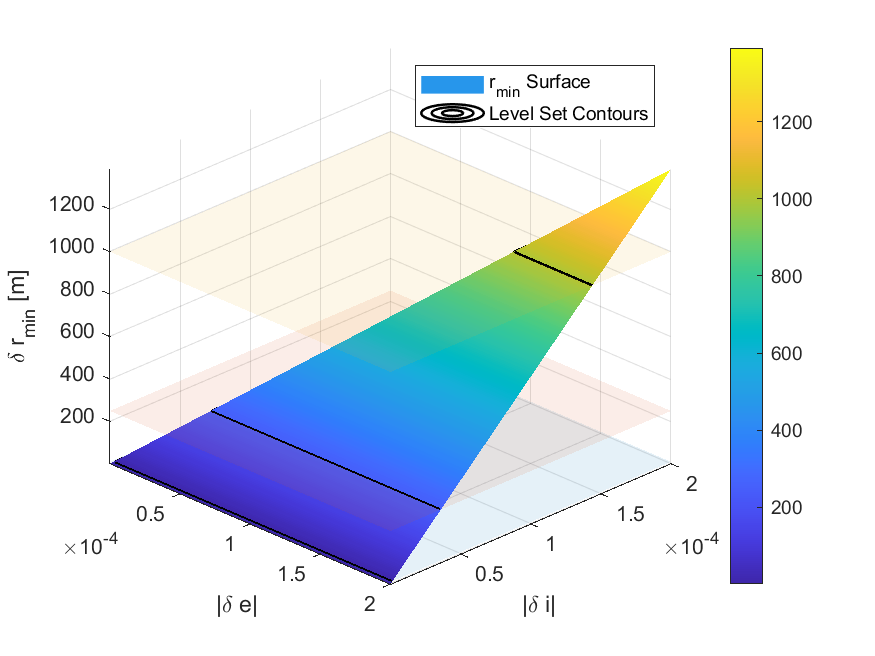
\includegraphics[width=0.75\linewidth]{sim/figures/PS5/min_dist_contour.png}
    \caption{Minimum distance contour over relative eccentricity and relative inclination}
    \label{fig:min_dist_contour}
\end{figure}
As such, $\delta e$ and $\delta i$ were chosen to be equal in magnitude for both SV2 and SV3 in order to give circular relative motion, which is helpful for maintaining the same distance throughout an orbit for the vision-based sensing on both spacecraft. Additionally, $\delta e$ and $\delta i$ were chosen to be antiparallel for SV3 (Docker) and parallel for SV2 (Watcher) to ensure that the Docker never blocks the Watcher's view of the Target by tilting the Docker's relative orbit perpendicular to the Watcher's.

\subsubsection{Formation Keeping Control Requirements}
For each station keeping mode, a keep-in region was defined for the relative eccentricity and relative inclination in order to ensure passive safety and maintain the allowable separations defined earlier. Due to the small size of the relative eccentricity and relative inclination vectors during our operational modes, a tight keep-in region of a circle with a 1-meter radius was used. 

This tight keep-in region dictates a tight relative position knowledge requirement: the Watcher's knowledge should be less than a meter and the Docker's should be less than a centimeter in order to allow for successful docking and servicing. Similarly, the velocity estimation of the Docker should be on order of mm/s.

Additionally, the actuation needed will be low-thrust, high-preicison with a low impulse bit on the order of mm/s, such as a cold gas thruster. Short, impulsive bursts will be used so to not disturb the attitude of the Docker and allow for precise control. 


\subsubsection{Reconfiguration Control Requirements}
For reconfiguration, there must always be passive safety, which is achieved through aligning the relative eccentricity and relative inclination vectors. Additionally the time to reconfigure, given in number of orbits, is prescribed for each mode below. These numbers were chosen to best illustrate the control behavior. In practice, the Approach Mode would take the longest time, especially in proximity operations where the maneuvers are small and need to be precise. 

\begin{table}[h!]
\centering
\begin{tabular}{|c|c|}
\hline
\textbf{Phase} & \textbf{Number of Orbits} \\
\hline
Mode 2 & 2 \\
Station-Keeping 2 & 3 \\
Mode 3 & 2 \\
Station-Keeping 3 & 3 \\
Mode 4 & 2 \\
\hline
\end{tabular}
\caption{Number of orbits spent in each mode and station-keeping phase} \label{tab:mode_durations}
\end{table}

\subsubsection{Choice of Actuators}
Two different types of actuators will be used. The first will be higher-thrust and lower specific impulse chemical propulsion for station keeping, phasing, and the approach. Electric propulsion is also an option here as it has higher specific impulse, but will not be used for now as impulsive delta-v's are simpler to model. The second kind of actuator used with be lower-thrust propulsion, such as cold-gas thrusters. These will be used for proximity and docking operations, as fine and accurate thrust control with small impulse bits is required. Cold gas thrusters will be used instead of hydrazine thrusters since they are less hazardous to work with. 

\subsubsection{Absolute and Relative Orbit Dynamics Models}
Two dynamics models are needed: the first will be the ground-truth and the second will actually run onboard the computationally-limited spacecraft. The absolute ground-truth will be given by numerical integration of the Fundamental Orbital Differential Equation (FODE) with J2 effects for the chief and both deputies. The relative ground-truth will be calculated by taking the differences in the absolute states and converting to the RTN and ROE representations. The onboard dynamics model cannot perform numerical integration as this would be too computationally-expensive. Instead, the absolute and onboard dynamics will be given by the analytical STM with J2 for ROE as outlined in Section \ref{sec:j2_analytical_roe}, which still needs to provide accuracy as it will be used for control. 

Implementing the ground-truth model in open-loop shows each desired mode in the RTN planes as shown in Figures \ref{fig:mode_1_rtn}, \ref{fig:mode_2_rtn}, \ref{fig:mode_3_rtn}. Note that Mode 4 is not shown because SV3 does not appear in the plots due to its ROE all being 0. This ground-truth model exhibits expected J2 perturbations with a drifting relative perigee. Also note how the inclinations of the relative orbits are offset in the NT projection due to the design choice of antiparallel relative eccentricity and relative inclination vectors of SV3. All of these modes exhibit passive safety as well. 

% --- Mode 1 ---
\begin{figure}[H]
    \centering
    \begin{subfigure}[b]{0.32\linewidth}
        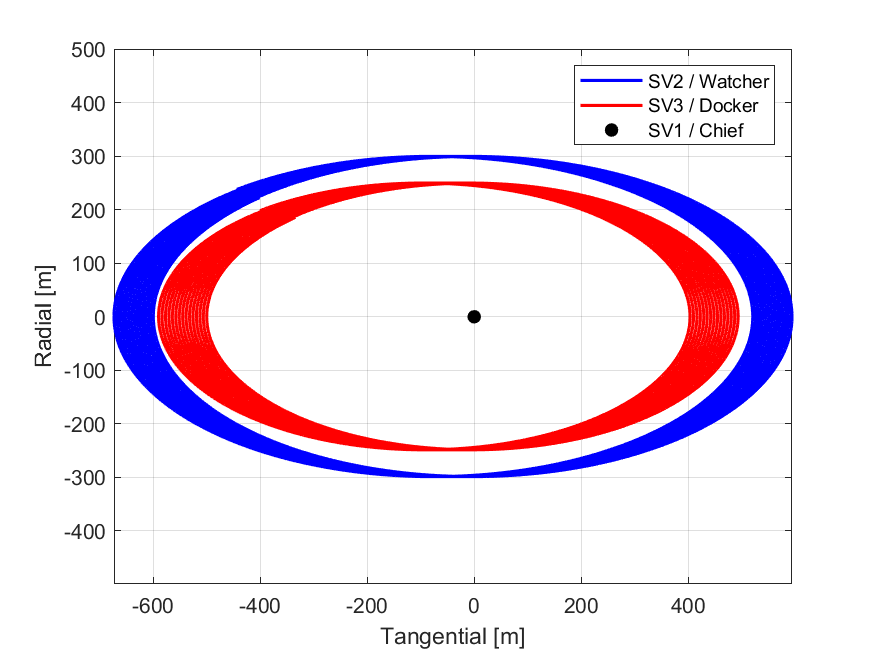
\includegraphics[width=\linewidth]{sim/figures/PS5/mode_1_RTN.png_RT.png}
        \caption{RT Projection}
        \label{fig:mode_1_rt}
    \end{subfigure}
    \begin{subfigure}[b]{0.32\linewidth}
        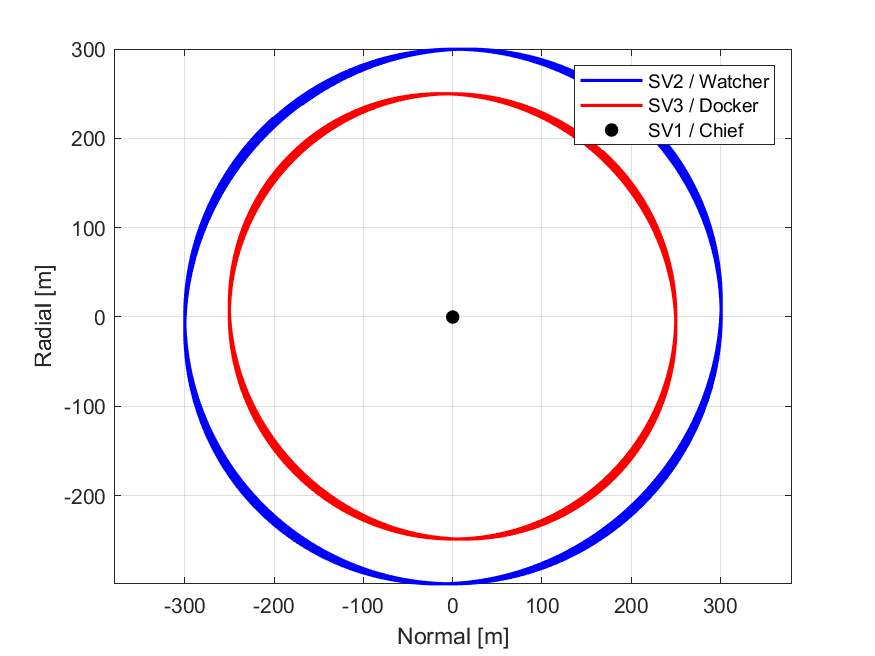
\includegraphics[width=\linewidth]{sim/figures/PS5/mode_1_RTN.png_RN.png}
        \caption{RN Projection}
        \label{fig:mode_1_rn}
    \end{subfigure}
    \begin{subfigure}[b]{0.32\linewidth}
        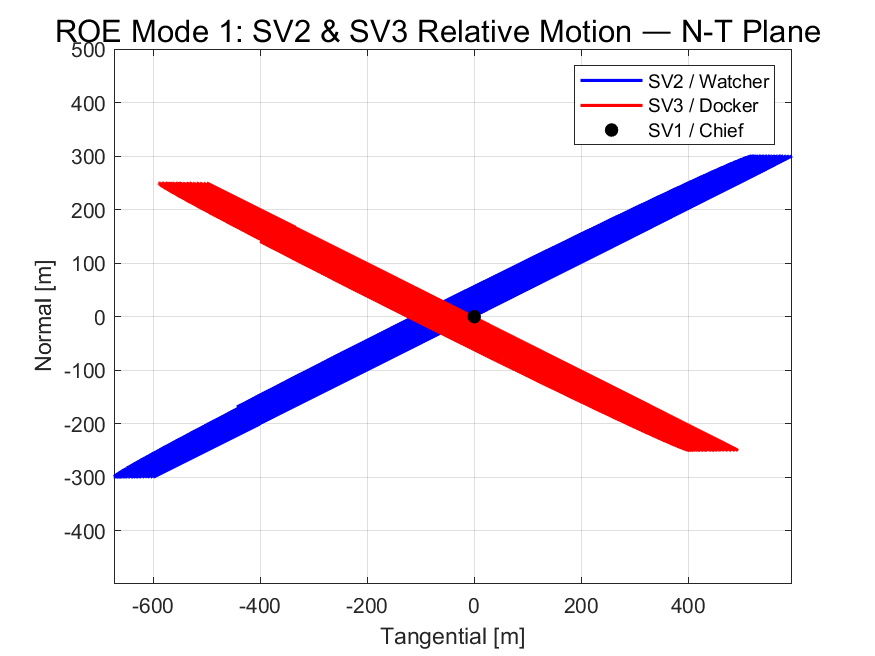
\includegraphics[width=\linewidth]{sim/figures/PS5/mode_1_RTN.png_NT.png}
        \caption{NT Projection}
        \label{fig:mode_1_nt}
    \end{subfigure}
    \caption{Mode 1 RTN Projections}
    \label{fig:mode_1_rtn}
\end{figure}

% --- Mode 2 ---
\begin{figure}[H]
    \centering
    \begin{subfigure}[b]{0.32\linewidth}
        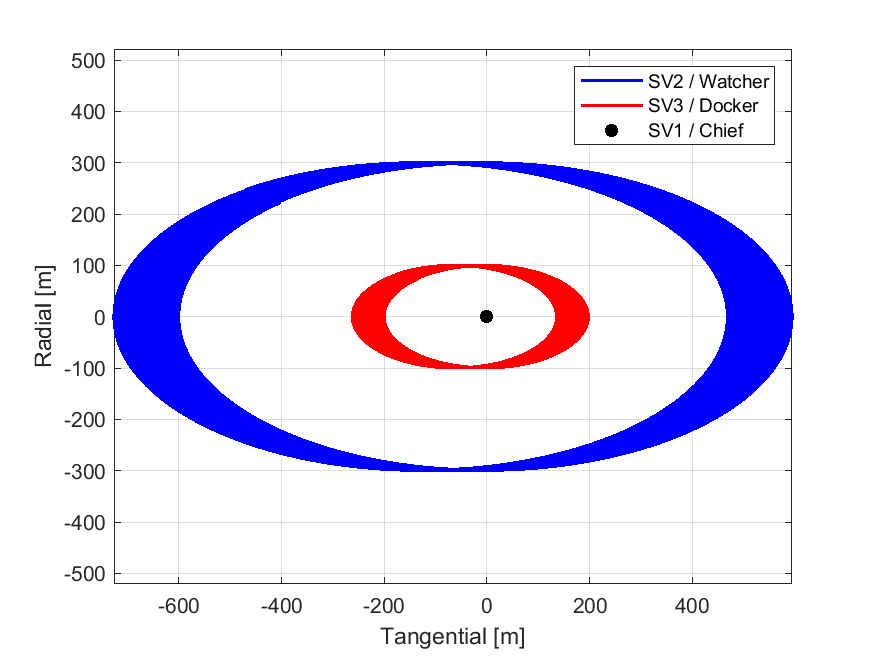
\includegraphics[width=\linewidth]{sim/figures/PS5/mode_2_RTN.png_RT.png}
        \caption{RT Projection}
        \label{fig:mode_2_rt}
    \end{subfigure}
    \begin{subfigure}[b]{0.32\linewidth}
        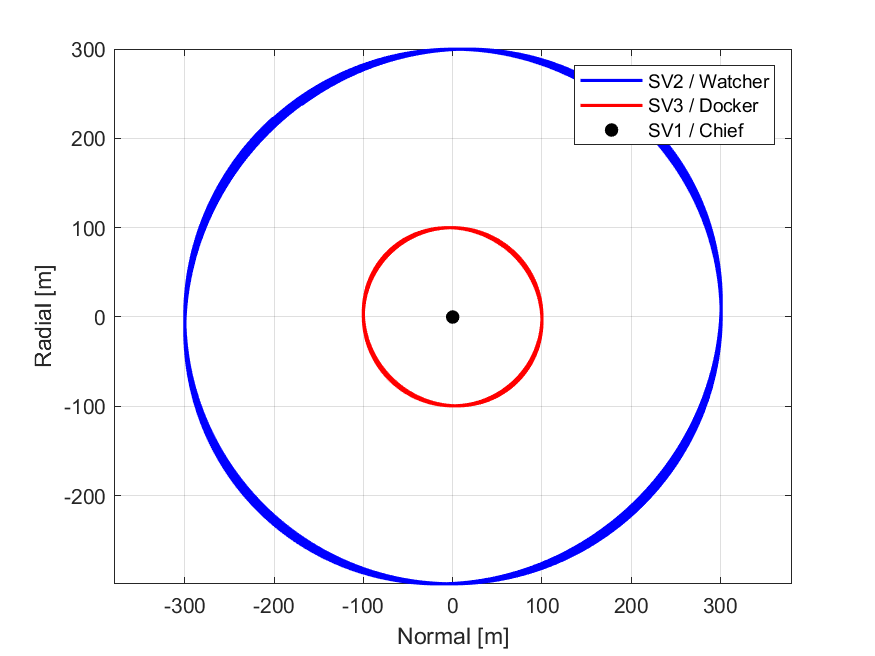
\includegraphics[width=\linewidth]{sim/figures/PS5/mode_2_RTN.png_RN.png}
        \caption{RN Projection}
        \label{fig:mode_2_rn}
    \end{subfigure}
    \begin{subfigure}[b]{0.32\linewidth}
        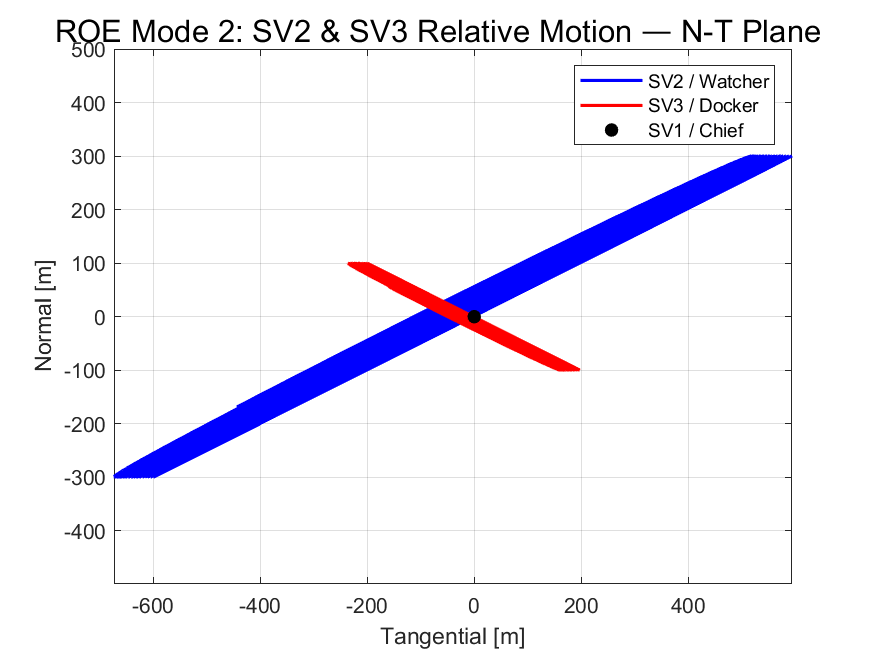
\includegraphics[width=\linewidth]{sim/figures/PS5/mode_2_RTN.png_NT.png}
        \caption{NT Projection}
        \label{fig:mode_2_nt}
    \end{subfigure}
    \caption{Mode 2 RTN Projections}
    \label{fig:mode_2_rtn}
\end{figure}

% --- Mode 3 ---
\begin{figure}[H]
    \centering
    \begin{subfigure}[b]{0.32\linewidth}
        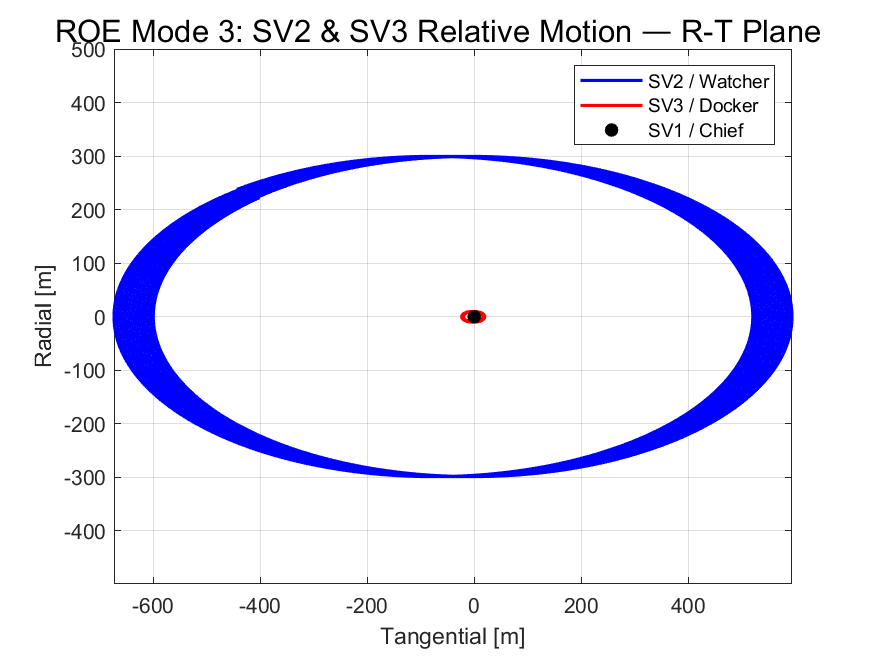
\includegraphics[width=\linewidth]{sim/figures/PS5/mode_3_RTN.png_RT.png}
        \caption{RT Projection}
        \label{fig:mode_3_rt}
    \end{subfigure}
    \begin{subfigure}[b]{0.32\linewidth}
        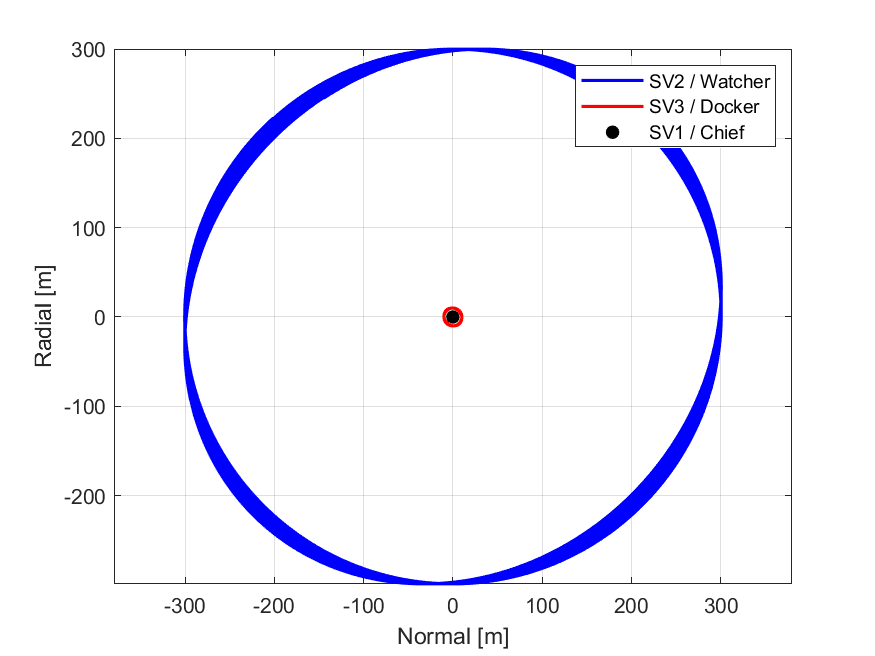
\includegraphics[width=\linewidth]{sim/figures/PS5/mode_3_RTN.png_RN.png}
        \caption{RN Projection}
        \label{fig:mode_3_rn}
    \end{subfigure}
    \begin{subfigure}[b]{0.32\linewidth}
        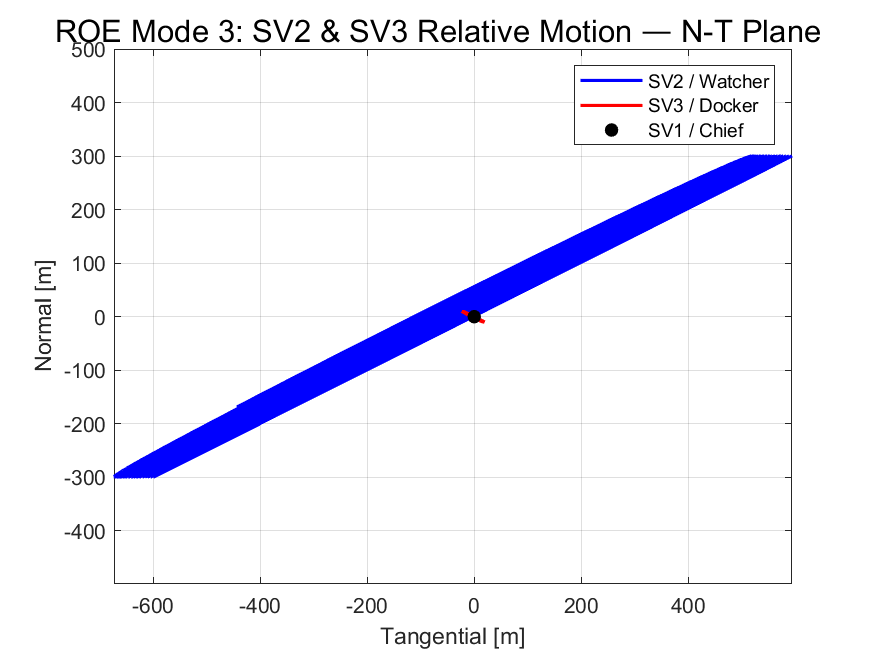
\includegraphics[width=\linewidth]{sim/figures/PS5/mode_3_RTN.png_NT.png}
        \caption{NT Projection}
        \label{fig:mode_3_nt}
    \end{subfigure}
    \caption{Mode 3 RTN Projections}
    \label{fig:mode_3_rtn}
\end{figure}

To verify that the STM is an acceptable model, it is compared in the ROE representation. As seen in Figures \ref{fig:roe_plane_compare_method} and \ref{fig:roe_time_compare_method} the STM aligns closely with the ground-truth Differences in FODE (Dif. FODE) method. The one notable exception is in the $\delta i_y$ case, although the error is very minimal.

\begin{figure}[H]
    \centering
    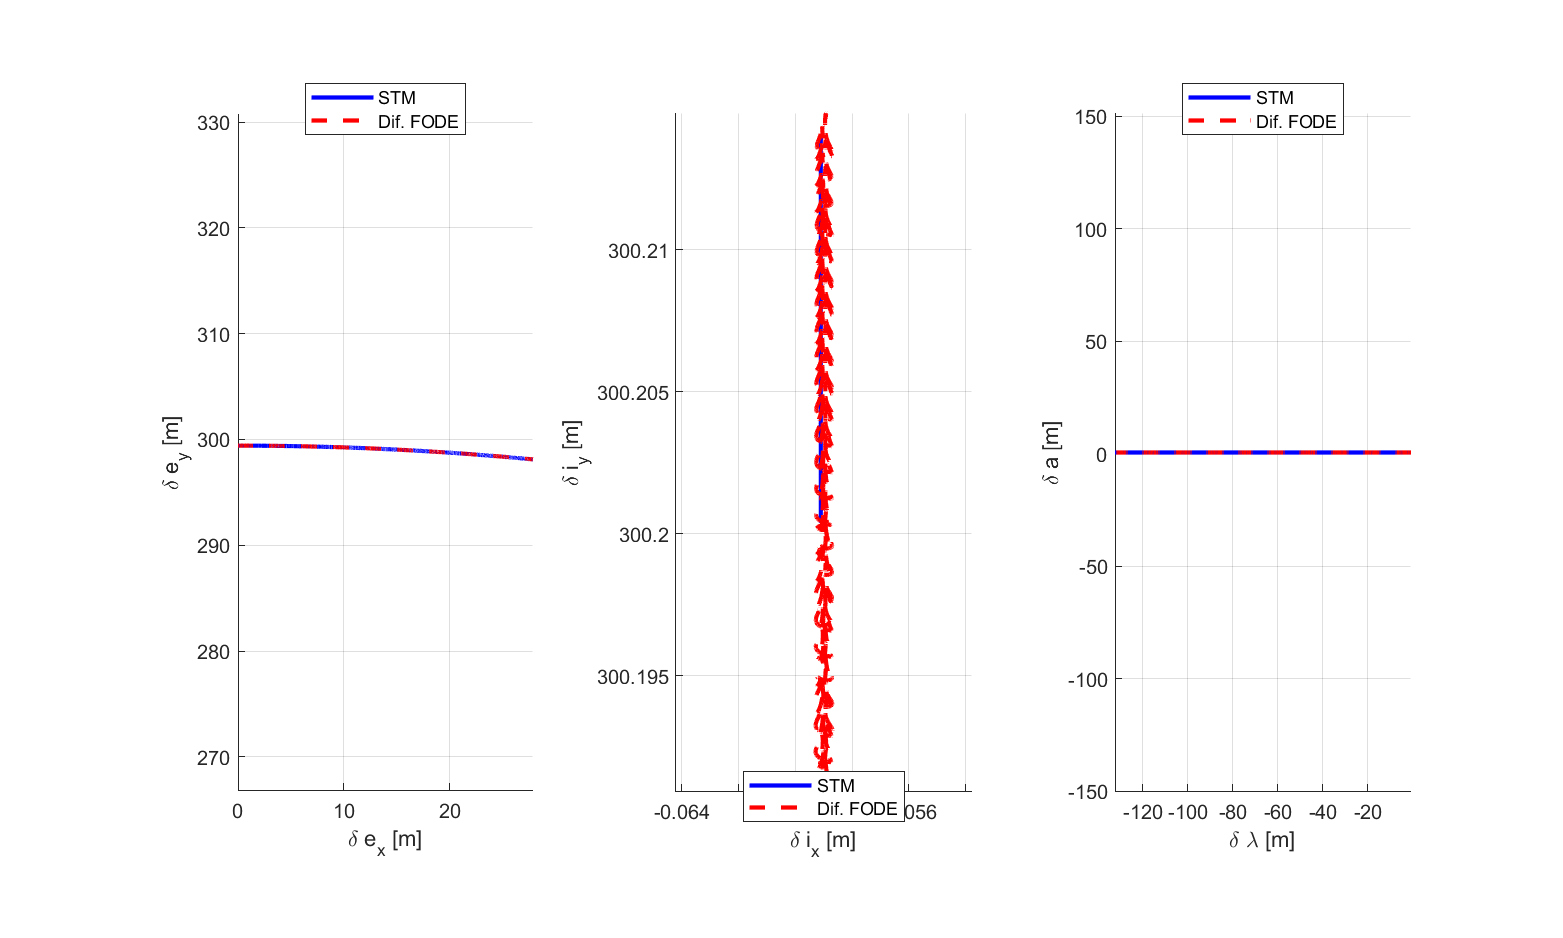
\includegraphics[width=0.75\linewidth]{sim/figures/PS5/mode_1_ROE_Planes.png}
    \caption{STM and Dif. FODE methods plotted in ROE planes}
    \label{fig:roe_plane_compare_method}
\end{figure}
\begin{figure}[H]
    \centering
    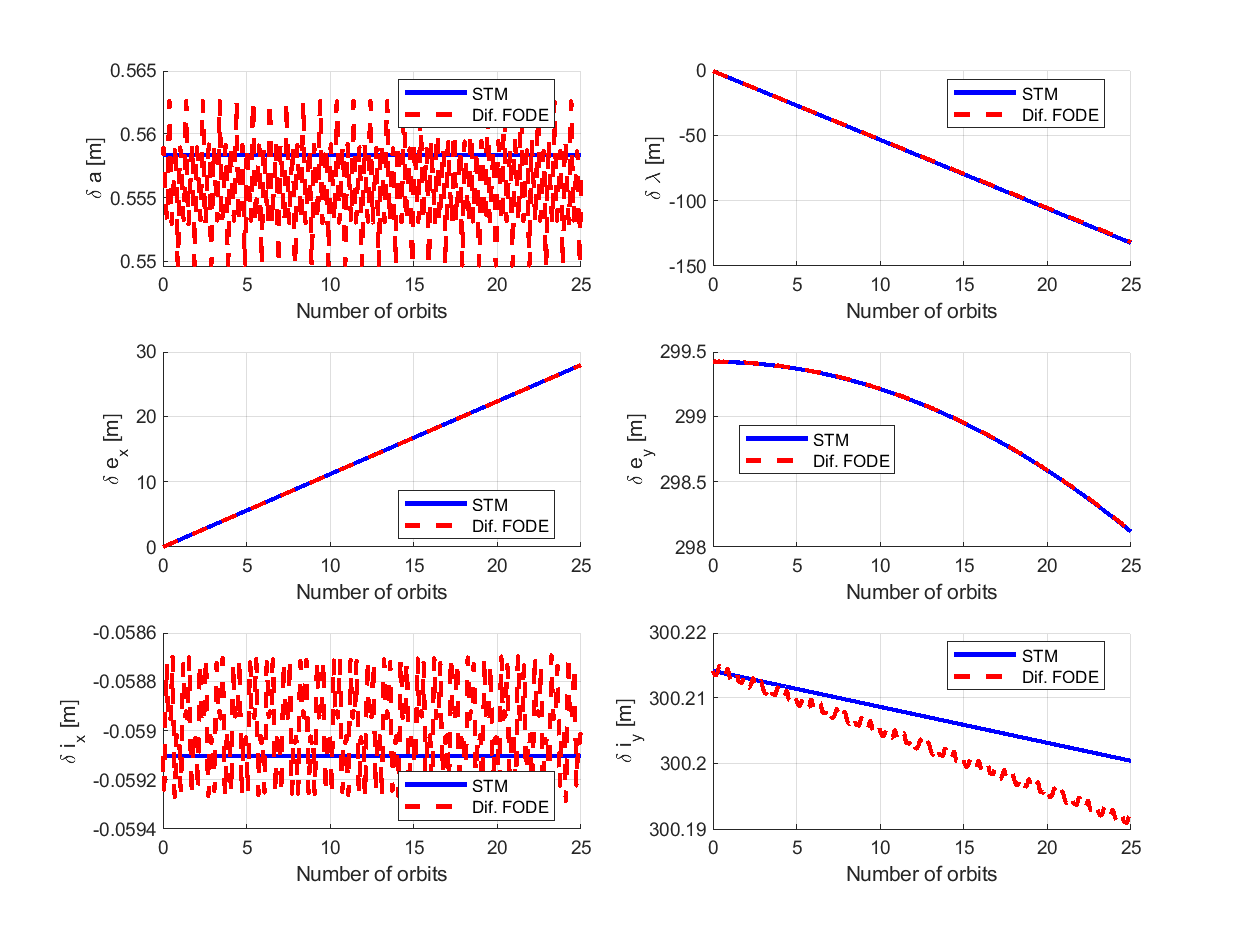
\includegraphics[width=0.75\linewidth]{sim/figures/PS5/mode_1_ROE_Time.png}
    \caption{STM and Dif. FODE methods plotted in ROE time history}
    \label{fig:roe_time_compare_method}
\end{figure}
\subsection{Impulsive Control Law}

\subsubsection{Control Method Considerations}

As highlighted in Section \ref{sec:control_objectives}, our system has four distinct operational modes, each with their own unique control accuracy and safety requirements. We also have control considerations for the maneuvers for transitioning between different modes.

Based on the requirements detailed in the previous section, we decided on the operational methods highlighted in Table \ref{tab:mode_control_methods}. Note here, that just the Docker (SV3) that performs the approach towards SV1, and so its control schemes change with time. SV2, on the other hand, keeps its original station through all modes, and does not perform any larger maneuvers (attitude maneuvers are not considered in this formulation).

\definecolor{lightgray}{gray}{0.9}

\begin{table}[ht]
    \centering
    \caption{Control Methods by Mode of Operation}
    \renewcommand{\arraystretch}{1.3}

    \begin{tabularx}{\textwidth}{|>{\raggedright\arraybackslash}p{0.13\textwidth}|%
                                      >{\raggedright\arraybackslash}p{0.13\textwidth}|%
                                      >{\raggedright\arraybackslash}p{0.12\textwidth}|%
                                      >{\raggedright\arraybackslash}p{0.12\textwidth}|%
                                      >{\raggedright\arraybackslash}p{0.12\textwidth}|%
                                      >{\raggedright\arraybackslash}X|}
        \rowcolor{lightgray}
        \hline
        \textbf{Mode of Operation} & \textbf{Tracked State} & \textbf{In-plane Control Method} & \textbf{Out-of-plane Control Method} & \textbf{Control Window} & \textbf{Reasoning} \\
        \hline
        General Station Keeping (SV2 always and SV3 Mode 1) & Relative orbital elements that provide passive safety & Pairs of along-track burns & Single impulse cross-track burn & Full duration of station-keeping (see Table \ref{tab:mode_durations}) & Simple efficient control methodology that does not require prior time allocation. \\
        \hline
        Approach Transfer (SV3 Mode 2) & Desired Mode 2 final ROE & Naive least squares control solution & Naive least squares control solution & Two orbits for transfer & Simple open-loop solution, merges in-plane and out-of-plane, no drift in $\delta \lambda$ \\
        \hline
        Proximity Maneuvers (SV3 Mode 3) & Desired Mode 3 final ROE & Radial impulse burns & Single-impulse cross-track burn & Two orbits for transfer & Provides tight control, no plume on target satellite. \\
        \hline
        Docked Station Keeping (SV3 Mode 4) & N/A (Docked State) & No in-plane control & No out-of-plane control & Service duration & Rigid-body docking eliminates relative motion; no active control required. \\
        \hline
    \end{tabularx}
    \label{tab:mode_control_methods}
\end{table}



\subsubsection{Control Maneuver Formulations}
Although we had the different ideas for control methodologies for the different modes, during the duration of this submission we were only able to get one method working exactly to meet our requirements: naive least squares. Two other methods were attempted: the relative orbit control impulse burn formulations in \cite{damicothesis}, and the closed-form control solution highlighted in \cite{chernick2021optimal}. However, the method from \cite{damicothesis} causes a drift in the $\delta \lambda$ that we were not able to close (likely with a third burn). We were also unable to complete a working implementation of the closed-form solution. Although these will be discussed in later submissions (to cover all the methods detailed in Table \ref{tab:mode_control_methods}), here we will primarily discuss the naive-least squares method.

The naive least-squares method works on the principle that a sequence of relative orbital elements can be related to each other with a linearized model that accounts for J2 perturbations, called a state transition matrix. This STM was previously stated in Equations \ref{eq:stm_matrix} and \ref{eq:state_transition_relation}. 

The change in relative orbital elements $\Delta \delta \alpha$ can also be related to the applied $\Delta v$ as \cite{chernick2021optimal}
\begin{align}
    \boldsymbol{\Delta \delta \alpha} = \Gamma\Delta \boldsymbol{v}
\end{align} \label{eq:delta_v_to+alpha}
Putting these together, we have a formulation for a set of control maneuvers $\Delta v$ required to achieve a desired change in relative orbital elements.
\begin{equation}
\Delta \delta \boldsymbol{\alpha} = \delta \boldsymbol{\alpha}(t_f) - \Phi_{f,0} \, \delta \boldsymbol{\alpha}(t_0)
= \sum_{k = 1}^{M} \Phi(t_k) \Gamma (t_k)  \delta \mathbf{v}_k
\end{equation}
From theoretical formulations, we adopt the standard of setting three equally-spaced in time $\Delta v$ impulses for in-plane maneuvers, or a single impulse burn $\Delta v$ for out-of-plane maneuvers.
For near-circular orbit, the transformation matrix $\Gamma$ is given simply by
\begin{align}
\Delta \delta \boldsymbol{\alpha}_k = \Gamma_k \delta \mathbf{v}_k = \frac{1}{na}
\begin{bmatrix}
0 & 2 & 0 \\
-2 & 0 & 0 \\
\sin(u_k) & 2\cos(u_k) & 0 \\
-\cos(u_k) & 2\sin(u_k) & 0 \\
0 & 0 & \cos(u_k) \\
0 & 0 & \sin(u_k)
\end{bmatrix}
\begin{bmatrix}
\delta v_R \\
\delta v_T \\
\delta v_N
\end{bmatrix}
\end{align}

where $\Delta v$ is in the RTN frame, and $a$ is the semi-major axis of the chief SV1. We can also relate the mean argument of latitude to the maneuver time using the formulation

\begin{align}
    u_k = t_{k} \left( n + \kappa \left( \eta P + Q \right) \right) + u_{0}
\end{align}

where $P, Q, \eta, \kappa$ are defined in Equation \ref{}.

The control maneuvers are solved by applying least-squares the linear system $Ax = b$ which we 



The comparison of the least-squares method with the lower-bound delta-v $\Delta v_{lb}$ is provided in Section \ref{sec:analysis_of_control}.




\subsubsection{Justificiation and Implementation of Control}

For implementing our method in simulation we utilized 
* FODE Dynamics model (segmented for control)
* Logic 


Separate from the primary simulation that implemented the different modes and maneuvers, we implemented a 


\begin{algorithm}[H]
\caption{Stationkeeping Simulation and Plotting}
\begin{algorithmic}[1]
\Procedure{SimAndPlotStationkeeping}{SV2\_modes, SV3\_modes, SV1\_OE\_init, SV2\_state\_init, SV3\_state\_init, SV1\_state\_init, $t_{\text{orbit}}$, $t_{\text{series}}$, fig\_path, title\_str}

\State Initialize time array, chief semi-major axis, and empty state histories
\State Extract nominal ROE for SV2 and SV3; define stationkeeping bounds
\State Compute desired eccentricity offsets using rotation angles

\For{each time step $t_i$ in $t_{\text{series}}$}
    \State Propagate SV1, SV2, SV3 states using RK4
    \State Convert SV2 and SV3 states to ROE w.r.t. SV1
    \State Extract orbital elements and mean argument of latitude

    \If{SV2 has not yet performed control}
        \If{eccentricity deviation exceeds threshold}
            \State Compute and store SV2 $\Delta v$ for eccentricity control
        \EndIf
        \If{inclination deviation exceeds threshold}
            \State Compute and store SV2 $\Delta v$ for inclination control
        \EndIf
    \EndIf

    \If{SV3 has not yet performed control}
        \If{eccentricity deviation exceeds threshold}
            \State Compute and store SV3 $\Delta v$ for eccentricity control
        \EndIf
        \If{inclination deviation exceeds threshold}
            \State Compute and store SV3 $\Delta v$ for inclination control
        \EndIf
    \EndIf

    \If{a planned SV2 $\Delta v$ is scheduled now}
        \State Apply $\Delta v$ to SV2 and remove it from queue
    \EndIf
    \If{a planned SV3 $\Delta v$ is scheduled now}
        \State Apply $\Delta v$ to SV3 and remove it from queue
    \EndIf
\EndFor

\State Convert SV2 and SV3 final states to RTN position relative to SV1
\State Plot RTN projections and ROE evolution over time
\EndProcedure
\end{algorithmic}
\end{algorithm}


For this submission, considerations of the delta-v budget, actuator implementation, sensor models, and disturbance models (apart from J2) are ignored. These other practical considerations will be incorporated in future submissions.

\subsubsection{Results and Analysis of Control Performance} \label{sec:analysis_of_control}

\begin{figure}
    \centering
    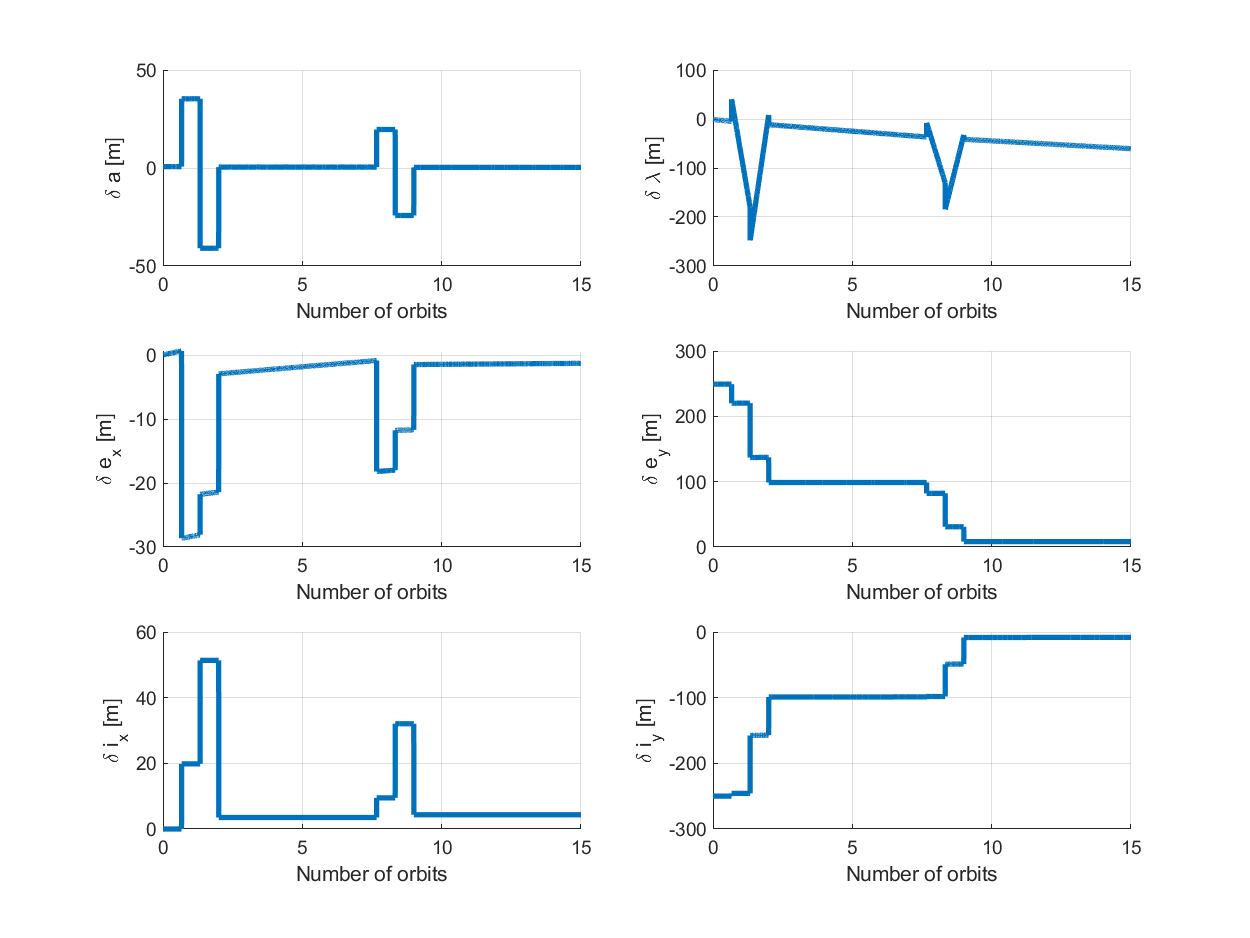
\includegraphics[width=0.5\linewidth]{sim/figures/PS5/ROE_over_time.png}
    \caption{Enter Caption}
    \label{fig:enter-label}
\end{figure}
\begin{figure}
    \centering
    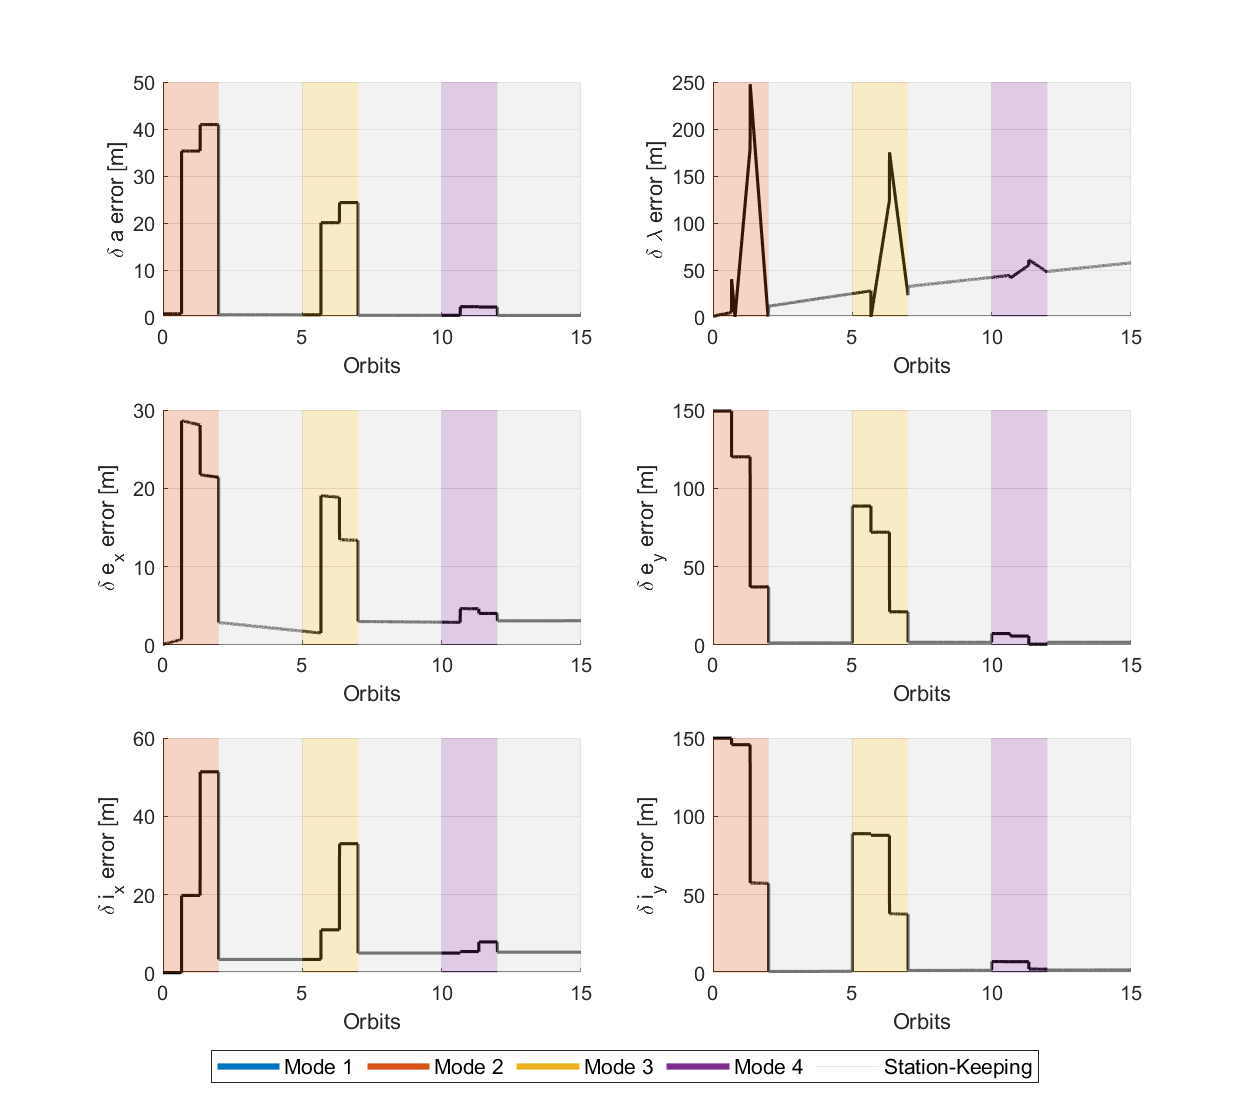
\includegraphics[width=0.5\linewidth]{sim/figures/PS5/ROE_error_over_time.png}
    \caption{Enter Caption}
    \label{fig:enter-label}
\end{figure}
\begin{figure}
    \centering
    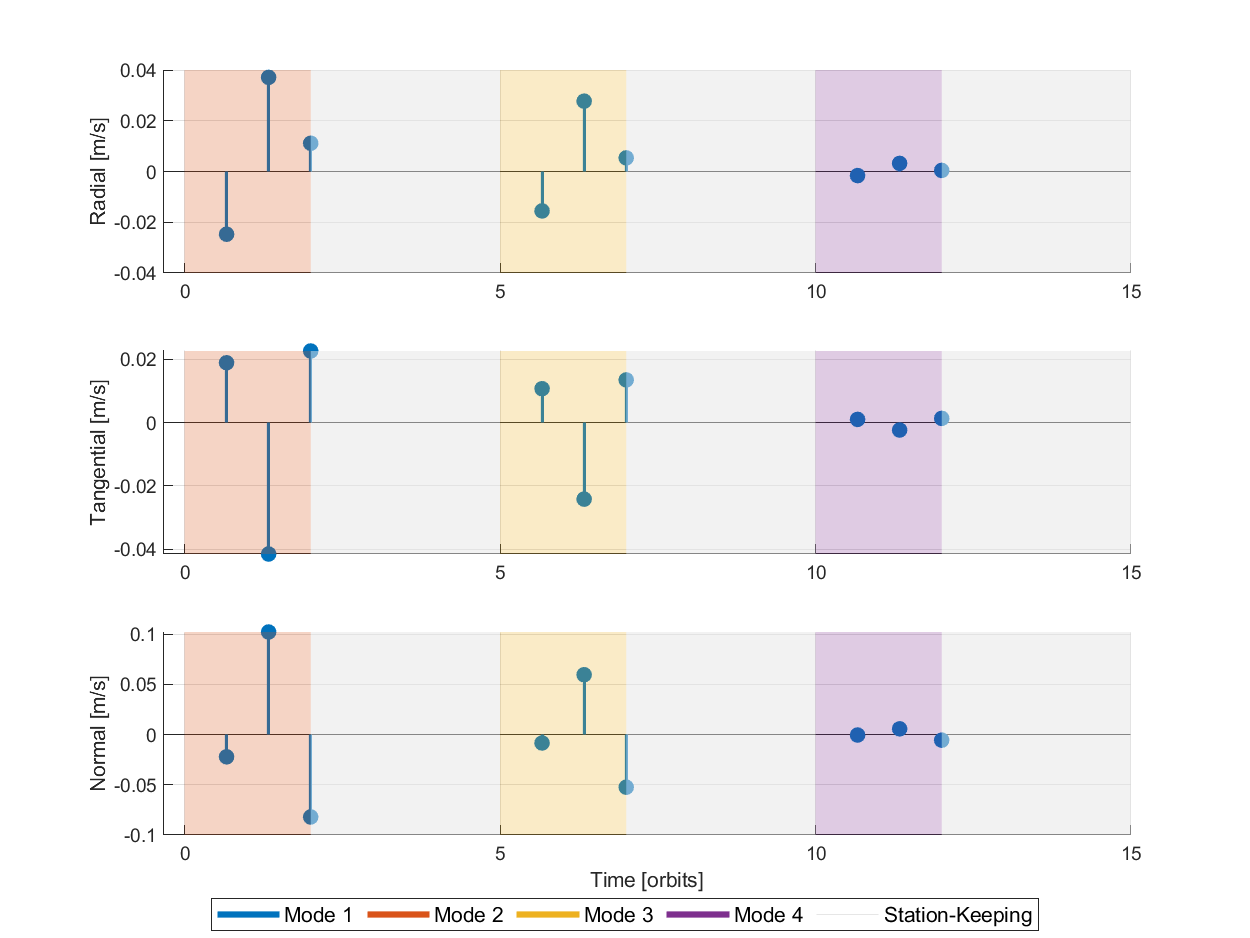
\includegraphics[width=0.5\linewidth]{sim/figures/PS5/delta_v_timeline.png}
    \caption{Enter Caption}
    \label{fig:enter-label}
\end{figure}

